\documentclass[]{article}
\usepackage{lmodern}
\usepackage{amssymb,amsmath}
\usepackage{ifxetex,ifluatex}
\usepackage{fixltx2e} % provides \textsubscript
\ifnum 0\ifxetex 1\fi\ifluatex 1\fi=0 % if pdftex
  \usepackage[T1]{fontenc}
  \usepackage[utf8]{inputenc}
\else % if luatex or xelatex
  \ifxetex
    \usepackage{mathspec}
    \usepackage{xltxtra,xunicode}
  \else
    \usepackage{fontspec}
  \fi
  \defaultfontfeatures{Mapping=tex-text,Scale=MatchLowercase}
  \newcommand{\euro}{€}
\fi
% use upquote if available, for straight quotes in verbatim environments
\IfFileExists{upquote.sty}{\usepackage{upquote}}{}
% use microtype if available
\IfFileExists{microtype.sty}{%
\usepackage{microtype}
\UseMicrotypeSet[protrusion]{basicmath} % disable protrusion for tt fonts
}{}
\ifxetex
  \usepackage[setpagesize=false, % page size defined by xetex
              unicode=false, % unicode breaks when used with xetex
              xetex]{hyperref}
\else
  \usepackage[unicode=true]{hyperref}
\fi
\usepackage[usenames,dvipsnames]{color}
\hypersetup{breaklinks=true,
            bookmarks=true,
            pdfauthor={},
            pdftitle={Matemàtiques 1r batxillerat científic},
            colorlinks=true,
            citecolor=blue,
            urlcolor=blue,
            linkcolor=magenta,
            pdfborder={0 0 0}}
\urlstyle{same}  % don't use monospace font for urls
\usepackage{graphicx,grffile}
\makeatletter
\def\maxwidth{\ifdim\Gin@nat@width>\linewidth\linewidth\else\Gin@nat@width\fi}
\def\maxheight{\ifdim\Gin@nat@height>\textheight\textheight\else\Gin@nat@height\fi}
\makeatother
% Scale images if necessary, so that they will not overflow the page
% margins by default, and it is still possible to overwrite the defaults
% using explicit options in \includegraphics[width, height, ...]{}
\setkeys{Gin}{width=\maxwidth,height=\maxheight,keepaspectratio}
\setlength{\parindent}{0pt}
\setlength{\parskip}{6pt plus 2pt minus 1pt}
\setlength{\emergencystretch}{3em}  % prevent overfull lines
\providecommand{\tightlist}{%
  \setlength{\itemsep}{0pt}\setlength{\parskip}{0pt}}
\setcounter{secnumdepth}{5}

\title{Matemàtiques 1r batxillerat científic}
\date{}

% Redefines (sub)paragraphs to behave more like sections
\ifx\paragraph\undefined\else
\let\oldparagraph\paragraph
\renewcommand{\paragraph}[1]{\oldparagraph{#1}\mbox{}}
\fi
\ifx\subparagraph\undefined\else
\let\oldsubparagraph\subparagraph
\renewcommand{\subparagraph}[1]{\oldsubparagraph{#1}\mbox{}}
\fi

\begin{document}
\maketitle

{
\hypersetup{linkcolor=black}
\setcounter{tocdepth}{3}
\tableofcontents
}
\textbf{Bloc 1: Nombres. Polinomis}

\begin{center}\rule{0.5\linewidth}{\linethickness}\end{center}

\begin{center}\rule{0.5\linewidth}{\linethickness}\end{center}

\begin{center}\rule{0.5\linewidth}{\linethickness}\end{center}

\begin{center}\rule{0.5\linewidth}{\linethickness}\end{center}

\section{Nombres reals}\label{nombres-reals}

\subsection{El conjunt dels nombres
reals}\label{el-conjunt-dels-nombres-reals}

Un \href{https://en.wikipedia.org/wiki/Real_number}{nombre real} és
aquell que es pot representar al llarg d'una recta contínua. Per
exemple, tots els nombres associats a mesures físiques (longitud, força,
pes, etc) són nombres reals.
\href{http://www.mathsisfun.com/numbers/real-numbers.html}{Exemples de
nombres reals} són: \(1\), \(-5\), \(\sqrt{3}\), \(\pi\), \(4'15\),
\(2'\overline{3}\), \(\frac{4}{5}\). Al conjunt dels nombres reals se li
dóna la lletra \textbf{\(\mathbb{R}\)}.

La
\href{https://ca.wikipedia.org/wiki/Recta_num\%C3\%A8rica}{\textbf{recta
numèrica}} està formada pel conjunt de tots els nombres reals. Els
nombres reals són un \textbf{conjunt ordenat} ja que donats dos nombres,
sempre podem determinar-ne el més gran: si \(a \gt b\) al
representar-los sobre la recta, \(a\) estarà a la dreta de \(b\).

Si recordeu de cursos anteriors, els nombres reals es dividien en
diversos subconjunts.

\begin{figure}[htbp]
\centering
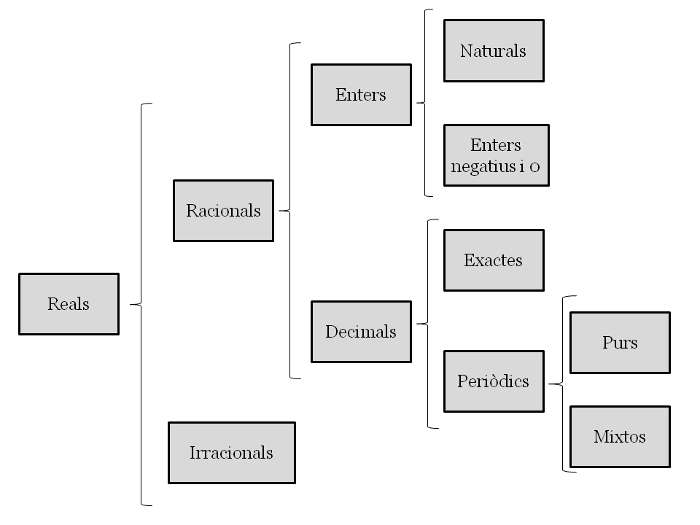
\includegraphics{img/classificacio_reals_1.png}
\caption{\emph{Classificació dels nombres reals}}
\end{figure}

Els nombres reals es divideixen en \textbf{nombres racionals}
\textbf{\(\mathbb{Q}\)}, que són aquells que es poden expressar
mitjançant una fracció i els \textbf{irracionals}
\textbf{\(\mathbb{I}\)}. Exemples de nombres racionals són
\(\frac{3}{4}\), \(2'5\) i \(0'\stackrel\frown{123}\). Els nombres
irracionals no es poden expressar com a fracció. El nombre \(\pi\) i
\(\sqrt{5}\) són nombres irracionals.

Els nombres \textbf{naturals} i els \textbf{enters} ja els coneixeu de
cursos anteriors:

\[\mathbb{N}=\{0, 1, 2, 3, 4,...\}\]
\[\mathbb{Z}=\{...-4, -3, -2, -1, 0, 1, 2, 3, 4,...\}\]

La relació entre els conjunts \(\mathbb{N}\), \(\mathbb{Z}\) i
\(\mathbb{Q}\) és la següent:
\(\mathbb{N} \subset \mathbb{Z} \subset \mathbb{Q}\). Això vol dir que
un nombre natural és alhora enter i racional, per exemple.

Els nombres \textbf{decimals} es divideixen en exactes i periòdics. Si
el període comença just després de la coma s'anomenen \textbf{periòdics
purs} (\(0'\stackrel\frown{3}=0'3333....\))i si hi ha alguna xifra que
no es repeteix abans s'anomenen \textbf{periòdics mixtes}
(\(0'2\stackrel\frown{45}=0'2454545....\)). Per a tots els nombres
decimals podem buscar la seva
\href{http://www.edu365.cat/eso/muds/matematiques/edad/eso4B/reales/q1_contenidos1b.htm}{fracció
generatriu}.

\subsection{Recta real}\label{recta-real}

Representar nombres sobre la recta real és ben fàcil si són racionals.
Si estem parlant d'enters, els sabrem situar sobre la recta sense
problema. Però què passa quan hem de situar per exemple, \(\frac{3}{7}\)
sobre la recta real? Hi ha varis mètodes. El mètode més ràpid és agafar
la unitat, fer-ne 7 parts i agafar-ne 3. El mètode més exacte és
utilitzant la tècnica de dibuixar un segment des del 0 amb un angle
qualsevol i dividir-lo en 7 parts iguals. Seguidament, uneixes l'última
part amb l'\(1\) de la recta real i traces línies paral.leles a aquesta
que passin per les altres divisions. Els punts d'intersecció amb la
recta real i aquestes rectes paral.leles et donaran les diferents
fraccions \(\frac{1}{7}\), \(\frac{2}{7}\), \(\frac{3}{7}\), etc. Si ho
desitges, pots descarregar-te el fitxer geogebra.

\begin{figure}[htbp]
\centering
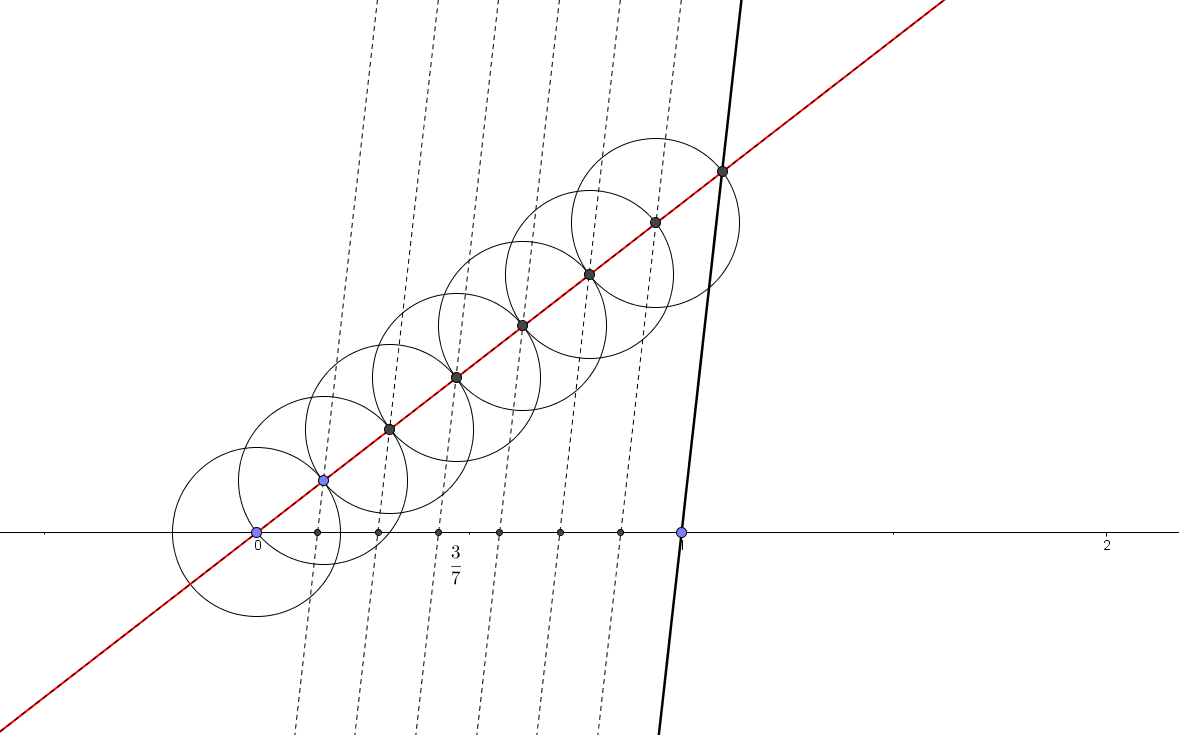
\includegraphics{img/fraccions_recta_real_1.png}
\caption{\emph{Representació de \(\frac{3}{7}\) sobre la recta real}}
\end{figure}

\subsubsection{Intervals}\label{intervals}

\subsubsection{Inequacions}\label{inequacions}

\subsection{Potències}\label{potuxe8ncies}

\subsubsection{Propietats}\label{propietats}

\subsection{Arrels}\label{arrels}

\subsubsection{Propietats}\label{propietats-1}

\subsubsection{Operacions}\label{operacions}

\subsubsection{Racionalització}\label{racionalitzaciuxf3}

\subsection{Logaritmes}\label{logaritmes}

\section{Trigonometria}\label{trigonometria}

\section{Nombres complexos}\label{nombres-complexos}

\section{Polinomis}\label{polinomis}

\textbf{Bloc 2: Geometria}

\begin{center}\rule{0.5\linewidth}{\linethickness}\end{center}

\begin{center}\rule{0.5\linewidth}{\linethickness}\end{center}

\begin{center}\rule{0.5\linewidth}{\linethickness}\end{center}

\begin{center}\rule{0.5\linewidth}{\linethickness}\end{center}

\section{Vectors en el pla}\label{vectors-en-el-pla}

\section{Rectes en el pla}\label{rectes-en-el-pla}

\section{Llocs geomètrics}\label{llocs-geomuxe8trics}

\textbf{Bloc 3: Funcions}

\begin{center}\rule{0.5\linewidth}{\linethickness}\end{center}

\begin{center}\rule{0.5\linewidth}{\linethickness}\end{center}

\begin{center}\rule{0.5\linewidth}{\linethickness}\end{center}

\begin{center}\rule{0.5\linewidth}{\linethickness}\end{center}

\section{Funcions}\label{funcions}

\section{Successions}\label{successions}

\section{Límits i continuïtat de
funcions}\label{luxedmits-i-continuuxeftat-de-funcions}

\section{Funció exponencial i
logarítmica}\label{funciuxf3-exponencial-i-logaruxedtmica}

\section{Funcions trigonomètriques}\label{funcions-trigonomuxe8triques}

\end{document}
